\chapter{Planning}
In dit hoofdstuk wordt de initiële planning beschreven, en daarbij de verschillende deadlines voor de op te leveren producten.
Verder wordt er een strokenplanning beschreven in hoofdstuk \ref{sec:strokenplanning}.
\section{Op te leveren producten}
De deadlines en concept versies van de verschillende eindproducten worden beschreven in Tabel \ref{tab:Deadline}.

\whitespace[2]
\begin{graphic}
	\captionsetup{type=table}
	\begin{tabularx}{\textwidth}{|l|l|X|}
		\hline
		\textbf{Op te leveren producten} & \textbf{Conceptversie}               & \textbf{Deadline}         \\
		\hline
		Plan van aanpak                  & vanwege tijdsdruk is dit niet gelukt & 6-10-2023                 \\
		\hline
		Onderzoeksverslag                & 1-11-2023                            & 15-11-2023                \\
		\hline
		Onderzoeksverslag (2de kans)     & 19-3-2023                            & 5-4-2024                  \\
		\hline
		Technische verslag                & 19-3-2023                            & 5-4-2024                  \\
		\hline
		Product                          & niet van toepassing                  & 5-4-2024                  \\
		\hline
		Presentatie                      & 15-4-2024                            & 29/30-4-2024 of 1-5-2024 \\
		\hline
	\end{tabularx}
	\caption{Deadlines en conceptversie inlever momenten}
	\label{tab:Deadline}
    \vspace{0.2cm}
\end{graphic}
\section{Strokenplanning}
\label{sec:strokenplanning}
In Figuur \ref{fig:StrokenPlanning}wordt de strokenplanning weergegeven, die een verwachting geeft van de verwachte voortgang van het project.
Deze planning omvat alle projectactiviteiten.

\whitespace[2]
\begin{graphic}
	\captionsetup{type=figure}
	\caption{Voorlopige Strokenplanning}
	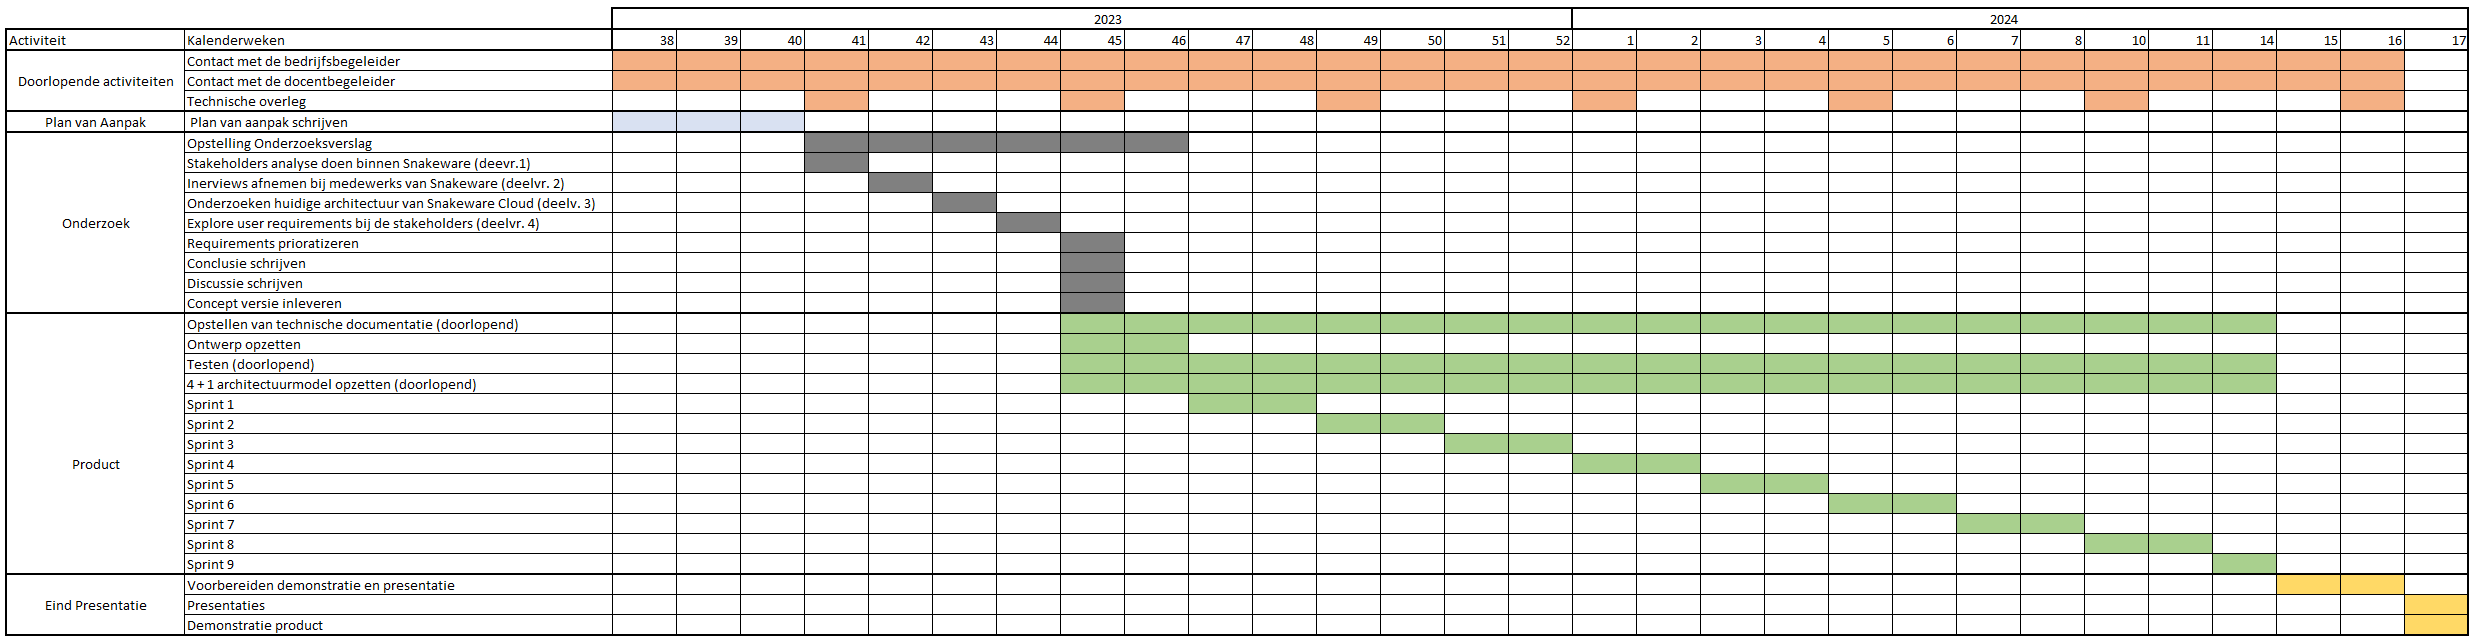
\includegraphics[scale=0.25]{StrokenPlanning}
	\label{fig:StrokenPlanning}
\end{graphic}
